
\documentclass[12pt, a4paper]{article}


%%%% Encodings

\usepackage[utf8]{inputenc} % encoding
\usepackage[english]{babel} % use special characters and also translates some elements within the document.

%%%% Misc

\usepackage{hyperref}       % Hyperlinks \url{url} or \href{url}{name}
\usepackage{parskip}        % \par starts on left (not idented)
\usepackage{tocbibind}      % Adds the bibliography to the table of contents (automatically)

% \usepackage[document]{ragged2e}  % Left-aligned (whole document)
% \begin{...} ... \end{...}   flushleft, flushright, center

%%%% Abstract

\usepackage{abstract}       % Abstract

% http://www.ctex.org/documents/packages/special/abstract.pdf
\renewcommand{\absnamepos}{flushleft} % \begin{abstract} \noindent ... \end{abstract}
\setlength{\absleftindent}{0pt}
\setlength{\absrightindent}{0pt}

%%%% Graphics

\usepackage{graphicx}
\graphicspath{ {./images/} } % directory to look up for graphics

% \begin{figure}[h]
%   \centering
%   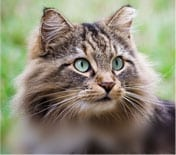
\includegraphics[scale=0.5]{cat}  % [width=\textwidth, height=4cm],
%   \caption{Example of a cat}
%   \label{fig:cat}
% \end{figure}

%%%% Math

\usepackage{amsmath}        % Math
\usepackage{amssymb}        % New symbols http://milde.users.sourceforge.net/LUCR/Math/mathpackages/amssymb-symbols.pdf
\usepackage{bm}             % $\bm{D + C}$

\usepackage{amsthm} % Math, \newtheorem, \proof, etc
% \begin{theorem}\label{t:label}  ...  \end{theorem}
% \begin{proof} ... \end{proof}
\theoremstyle{plain} % default
\newtheorem{theorem}{Theorem}[section]
\newtheorem{corollary}{Corollary}[theorem]  % Numering depends on the current section (instead of global)
\newtheorem{lemma}[theorem]{Lemma} % Shares numeration with theorem.
\theoremstyle{definition}
\newtheorem{definition}{Definition}[section]
\theoremstyle{remark}
\newtheorem*{remark}{Remark}

% Defines a new environment to write your or claim - proof
\newenvironment{claim}[1]{\par\noindent\underline{Claim:}\space#1}{}
\newenvironment{claimproof}[1]{\par\noindent\underline{Proof:}\space#1}{\hfill $\blacksquare$}

%%%% Code/Pseudo-code

\usepackage{minted} % Code listing
% \mint{html}|<h2>Something <b>here</b></h2>|
% \inputminted{octave}{BitXorMatrix.m}

%\begin{listing}[H]
  %\begin{minted}[xleftmargin=20pt,linenos,bgcolor=codegray]{haskell}
  %\end{minted}
  %\caption{Example of a listing.}
  %\label{lst:example} % You can reference it by \ref{lst:example}
%\end{listing}

\newcommand{\code}[1]{\texttt{#1}} % Define \code{foo.hs} environment

\usepackage[ruled,vlined]{algorithm2e} % pseudo-code http://tug.ctan.org/macros/latex/contrib/algorithm2e/doc/algorithm2e.pdf

%%%% Colors

\usepackage{xcolor}         % Colours \definecolor, \color{codegray}
\definecolor{codegray}{rgb}{0.9, 0.9, 0.9}
% \color{codegray} ... ...
% \textcolor{red}{easily}

%%%% Math

%\makeglossaries % before entries

%\newglossaryentry{latex}{
    %name=latex,
    %description={Is a mark up language specially suited
    %for scientific documents}
%}

% Referene to a glossary \gls{latex}
% Print glossaries \printglossaries

\usepackage[acronym]{glossaries} %

% \acrshort{name}
% \acrfull{name}
% \newacronym{foo}{arcshort}{acrfull}

\usepackage{enumitem} % \begin{enumerate}[label=(\alph*)]



\usepackage{fancyhdr}
\pagestyle{fancy}
\fancyhf{}
\rhead{Arnau Abella}
\lhead{Randomized Algorithms - UPC}
\rfoot{Page \thepage}

\title{%
  \vspace{-10ex}
  RA: An Exploratory Assignment on Minimum Spanning Trees
}
\author{%
  Arnau Abella \\
  \large{Universitat Polit\`ecnica de Catalunya}
}
\date{\today}

\begin{document}
\maketitle

%%%%%%%%%%%%%%%%%%%%

\vspace{5ex}

%In addition, you should write one or two pages discussing your experiments in more depth. The discussion should reflect what you have learned from this assignment and might address the following topics.

%* What minimmum spanning tree algorithm did you use, and why?
%* What is the running time of your algorithm?
%* If you chose to throw away edges, how did you determine `k(n)`, and how effective was this approach?
%* Can you give a rought explanation for your results? (The limiting behaviour as `n` grows large can be proven rigorously, but it is very difficult; you need not attempt to prove any exact result.)
%* Did you have any interesting experiences with the random number generator? Do you trust it?

\begin{algorithm}[H]
  \SetAlgoLined
  \DontPrintSemicolon
  % \LinesNumbered
  \SetKwInput{Input}{Input}
  \SetKwInput{Output}{Output}
  \Input{An undirected weighted graph $G = (V,E)$}
  \Output{The minimum spanning tree of the input graph $G$}
  \ForEach{$v \in V$}{
    $key(v) = \infty$\;
    $parent(v) = NIL$\;
  }
  $key(r) = 0$ \tcp*[r]{Pick \textit{u.a.r.} the initial vertex $r \in V$}
  $Q = V$\;
  \While{$Q \neq \emptyset$}{
    $u = EXTRACT-MIN(Q)$\;
    \ForEach{$v \in ADJ(u)$}{
      \If{$v \in Q$ and $w(u,v) < key(v)$}{
        $key(v) = w(u,v)$\;
        $parent(v) = u$\;
      }
    }
  }

  % \Return{$w$}\;
  \caption{Minimum Spanning Tree Prim's Algorithm}
\end{algorithm}


benchmarked prim/small
time                 8.100 ms   (7.960 ms .. 8.213 ms)
                     0.996 R²   (0.991 R² .. 0.999 R²)
mean                 8.358 ms   (8.278 ms .. 8.505 ms)
std dev              327.8 μs   (232.6 μs .. 476.6 μs)
variance introduced by outliers: 14% (moderately inflated)

benchmarking prim/medium ... took 22.24 s, total 56 iterations
benchmarked prim/medium
time                 406.0 ms   (401.9 ms .. 410.3 ms)
                     1.000 R²   (1.000 R² .. 1.000 R²)
mean                 391.9 ms   (383.9 ms .. 396.5 ms)
std dev              10.33 ms   (6.268 ms .. 15.21 ms)

benchmarking prim/big ... took 8.749 s, total 56 iterations
benchmarked prim/big
time                 153.6 ms   (151.9 ms .. 155.2 ms)
                     1.000 R²   (0.999 R² .. 1.000 R²)
mean                 150.3 ms   (148.2 ms .. 151.8 ms)
std dev              3.178 ms   (1.309 ms .. 4.035 ms)

benchmarking prim/bigger ... took 52.57 s, total 56 iterations
benchmarked prim/bigger
time                 943.1 ms   (937.4 ms .. 948.9 ms)
                     1.000 R²   (1.000 R² .. 1.000 R²)
mean                 934.4 ms   (920.9 ms .. 940.1 ms)
std dev              14.24 ms   (4.305 ms .. 23.30 ms)

%%%%%%%%%%%%%%%%%%%%
\end{document}
